\documentclass{standalone}
\usepackage{tikz}
\usetikzlibrary{patterns, positioning}

\begin{document}
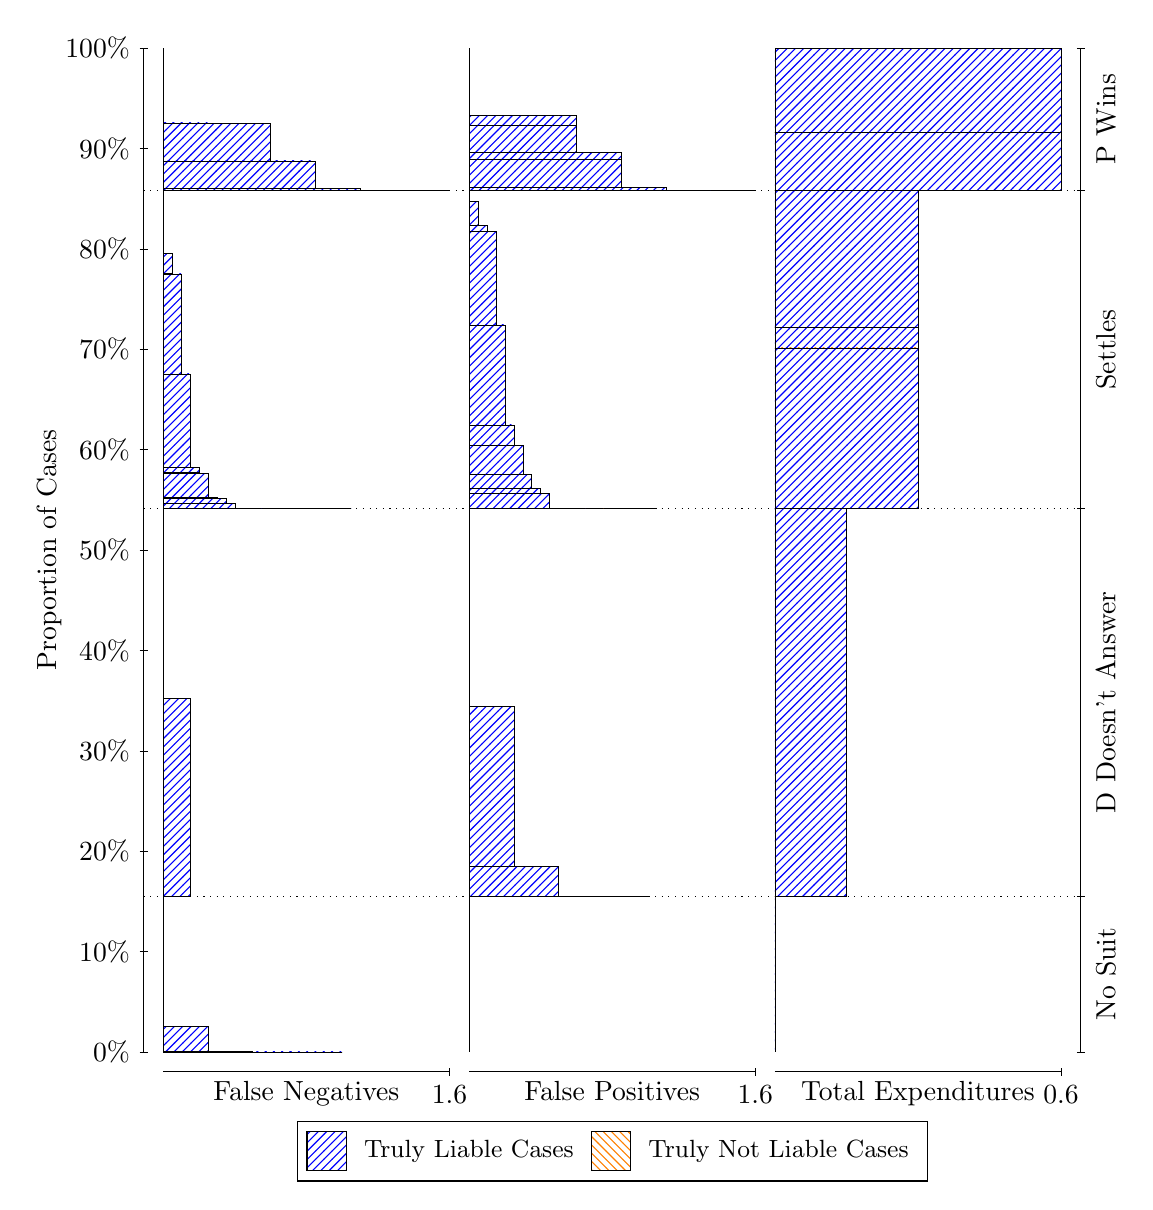
\begin{tikzpicture}
\draw[black, very thin] (1.5,1.75) -- (1.5,14.5);
\node[rotate=90, anchor=center] at (0.3, 8.125) {Proportion of Cases};
\draw[black, very thin] (1.45,1.75) -- (1.55,1.75);
\node[anchor=east] at (1.45, 1.75) {0\%};
\draw[black, very thin] (1.45,3.025) -- (1.55,3.025);
\node[anchor=east] at (1.45, 3.025) {10\%};
\draw[black, very thin] (1.45,4.3) -- (1.55,4.3);
\node[anchor=east] at (1.45, 4.3) {20\%};
\draw[black, very thin] (1.45,5.575) -- (1.55,5.575);
\node[anchor=east] at (1.45, 5.575) {30\%};
\draw[black, very thin] (1.45,6.85) -- (1.55,6.85);
\node[anchor=east] at (1.45, 6.85) {40\%};
\draw[black, very thin] (1.45,8.125) -- (1.55,8.125);
\node[anchor=east] at (1.45, 8.125) {50\%};
\draw[black, very thin] (1.45,9.4) -- (1.55,9.4);
\node[anchor=east] at (1.45, 9.4) {60\%};
\draw[black, very thin] (1.45,10.675) -- (1.55,10.675);
\node[anchor=east] at (1.45, 10.675) {70\%};
\draw[black, very thin] (1.45,11.95) -- (1.55,11.95);
\node[anchor=east] at (1.45, 11.95) {80\%};
\draw[black, very thin] (1.45,13.225) -- (1.55,13.225);
\node[anchor=east] at (1.45, 13.225) {90\%};
\draw[black, very thin] (1.45,14.5) -- (1.55,14.5);
\node[anchor=east] at (1.45, 14.5) {100\%};

\draw[black, very thin] (13.4,1.75) -- (13.4,14.5);
\draw[black, very thin] (13.35,1.75) -- (13.45,1.75);
\node[anchor=west] at (13.35, 1.75) {};
\draw[black, very thin] (13.35,3.7262) -- (13.45,3.7262);
\node[anchor=west] at (13.35, 3.7262) {};
\draw[black, very thin] (13.35,8.6515) -- (13.45,8.6515);
\node[anchor=west] at (13.35, 8.6515) {};
\draw[black, very thin] (13.35,12.695) -- (13.45,12.695);
\node[anchor=west] at (13.35, 12.695) {};
\draw[black, very thin] (13.35,14.5) -- (13.45,14.5);
\node[anchor=west] at (13.35, 14.5) {};

\draw[black, very thin, pattern color=blue, pattern=north east lines] (1.75,1.75) rectangle (4.0208,1.75);
\draw[black, very thin, pattern color=blue, pattern=north east lines] (1.75,1.75) rectangle (3.4531,1.75);
\draw[black, very thin, pattern color=blue, pattern=north east lines] (1.75,1.75) rectangle (2.8854,1.7528);
\draw[black, very thin, pattern color=blue, pattern=north east lines] (1.75,1.7528) rectangle (2.3177,2.0736);
\draw[black, very thin, pattern color=orange, pattern=north west lines] (1.75,2.0736) rectangle (1.75,2.0736);
\draw[black, very thin, pattern color=blue, pattern=north east lines] (1.75,2.0736) rectangle (1.75,3.7262);
\draw[black, very thin, pattern color=blue, pattern=north east lines] (1.75,3.7262) rectangle (2.0906,6.2407);
\draw[black, very thin, pattern color=orange, pattern=north west lines] (1.75,6.2407) rectangle (1.75,6.2407);
\draw[black, very thin, pattern color=blue, pattern=north east lines] (1.75,6.2407) rectangle (1.75,8.6515);
\draw[black, very thin, pattern color=blue, pattern=north east lines] (1.75,8.6515) rectangle (4.1344,8.6515);
\draw[black, very thin, pattern color=blue, pattern=north east lines] (1.75,8.6515) rectangle (3.9073,8.6515);
\draw[black, very thin, pattern color=blue, pattern=north east lines] (1.75,8.6515) rectangle (3.6802,8.6515);
\draw[black, very thin, pattern color=blue, pattern=north east lines] (1.75,8.6515) rectangle (3.5667,8.6515);
\draw[black, very thin, pattern color=blue, pattern=north east lines] (1.75,8.6515) rectangle (3.4531,8.6515);
\draw[black, very thin, pattern color=blue, pattern=north east lines] (1.75,8.6515) rectangle (3.3396,8.6515);
\draw[black, very thin, pattern color=blue, pattern=north east lines] (1.75,8.6515) rectangle (3.226,8.6515);
\draw[black, very thin, pattern color=blue, pattern=north east lines] (1.75,8.6515) rectangle (3.1125,8.6515);
\draw[black, very thin, pattern color=blue, pattern=north east lines] (1.75,8.6515) rectangle (2.999,8.6515);
\draw[black, very thin, pattern color=blue, pattern=north east lines] (1.75,8.6515) rectangle (2.8854,8.6521);
\draw[black, very thin, pattern color=blue, pattern=north east lines] (1.75,8.6521) rectangle (2.7719,8.6521);
\draw[black, very thin, pattern color=blue, pattern=north east lines] (1.75,8.6521) rectangle (2.7719,8.6522);
\draw[black, very thin, pattern color=blue, pattern=north east lines] (1.75,8.6522) rectangle (2.6583,8.7163);
\draw[black, very thin, pattern color=blue, pattern=north east lines] (1.75,8.7163) rectangle (2.5448,8.78);
\draw[black, very thin, pattern color=blue, pattern=north east lines] (1.75,8.78) rectangle (2.4312,8.7802);
\draw[black, very thin, pattern color=blue, pattern=north east lines] (1.75,8.7802) rectangle (2.4312,8.7898);
\draw[black, very thin, pattern color=blue, pattern=north east lines] (1.75,8.7898) rectangle (2.3177,9.0949);
\draw[black, very thin, pattern color=blue, pattern=north east lines] (1.75,9.0949) rectangle (2.2042,9.1133);
\draw[black, very thin, pattern color=blue, pattern=north east lines] (1.75,9.1133) rectangle (2.2042,9.1717);
\draw[black, very thin, pattern color=blue, pattern=north east lines] (1.75,9.1717) rectangle (2.0906,10.361);
\draw[black, very thin, pattern color=blue, pattern=north east lines] (1.75,10.361) rectangle (1.9771,11.633);
\draw[black, very thin, pattern color=blue, pattern=north east lines] (1.75,11.633) rectangle (1.8635,11.637);
\draw[black, very thin, pattern color=blue, pattern=north east lines] (1.75,11.637) rectangle (1.8635,11.892);
\draw[black, very thin, pattern color=orange, pattern=north west lines] (1.75,11.892) rectangle (1.75,11.892);
\draw[black, very thin, pattern color=blue, pattern=north east lines] (1.75,11.892) rectangle (1.75,12.695);
\draw[black, very thin, pattern color=blue, pattern=north east lines] (1.75,12.695) rectangle (5.3833,12.695);
\draw[black, very thin, pattern color=blue, pattern=north east lines] (1.75,12.695) rectangle (4.8156,12.695);
\draw[black, very thin, pattern color=blue, pattern=north east lines] (1.75,12.695) rectangle (4.2479,12.717);
\draw[black, very thin, pattern color=blue, pattern=north east lines] (1.75,12.717) rectangle (3.6802,13.066);
\draw[black, very thin, pattern color=blue, pattern=north east lines] (1.75,13.066) rectangle (3.4531,13.066);
\draw[black, very thin, pattern color=blue, pattern=north east lines] (1.75,13.066) rectangle (3.1125,13.547);
\draw[black, very thin, pattern color=blue, pattern=north east lines] (1.75,13.547) rectangle (2.8854,13.547);
\draw[black, very thin, pattern color=blue, pattern=north east lines] (1.75,13.547) rectangle (2.5448,13.547);
\draw[black, very thin, pattern color=blue, pattern=north east lines] (1.75,13.547) rectangle (2.3177,13.55);
\draw[black, very thin, pattern color=blue, pattern=north east lines] (1.75,13.55) rectangle (1.9771,13.55);
\draw[black, very thin, pattern color=orange, pattern=north west lines] (1.75,13.55) rectangle (1.75,13.55);
\draw[black, very thin, pattern color=blue, pattern=north east lines] (1.75,13.55) rectangle (1.75,14.5);
\draw[black, very thin, pattern color=orange, pattern=north west lines] (5.6333,1.75) rectangle (5.6333,1.75);
\draw[black, very thin, pattern color=blue, pattern=north east lines] (5.6333,1.75) rectangle (5.6333,3.7262);
\draw[black, very thin, pattern color=orange, pattern=north west lines] (5.6333,3.7262) rectangle (7.9042,3.7262);
\draw[black, very thin, pattern color=blue, pattern=north east lines] (5.6333,3.7262) rectangle (7.9042,3.7262);
\draw[black, very thin, pattern color=blue, pattern=north east lines] (5.6333,3.7262) rectangle (7.3365,3.7291);
\draw[black, very thin, pattern color=blue, pattern=north east lines] (5.6333,3.7291) rectangle (6.7687,4.1068);
\draw[black, very thin, pattern color=blue, pattern=north east lines] (5.6333,4.1068) rectangle (6.201,6.137);
\draw[black, very thin, pattern color=blue, pattern=north east lines] (5.6333,6.137) rectangle (5.6333,8.6515);
\draw[black, very thin, pattern color=orange, pattern=north west lines] (5.6333,8.6515) rectangle (8.0177,8.6515);
\draw[black, very thin, pattern color=blue, pattern=north east lines] (5.6333,8.6515) rectangle (8.0177,8.6515);
\draw[black, very thin, pattern color=orange, pattern=north west lines] (5.6333,8.6515) rectangle (7.5635,8.6515);
\draw[black, very thin, pattern color=blue, pattern=north east lines] (5.6333,8.6515) rectangle (7.5635,8.6515);
\draw[black, very thin, pattern color=blue, pattern=north east lines] (5.6333,8.6515) rectangle (7.45,8.6515);
\draw[black, very thin, pattern color=orange, pattern=north west lines] (5.6333,8.6515) rectangle (7.3365,8.6515);
\draw[black, very thin, pattern color=blue, pattern=north east lines] (5.6333,8.6515) rectangle (7.3365,8.6515);
\draw[black, very thin, pattern color=orange, pattern=north west lines] (5.6333,8.6515) rectangle (7.1094,8.6515);
\draw[black, very thin, pattern color=blue, pattern=north east lines] (5.6333,8.6515) rectangle (7.1094,8.6515);
\draw[black, very thin, pattern color=blue, pattern=north east lines] (5.6333,8.6515) rectangle (6.9958,8.6515);
\draw[black, very thin, pattern color=orange, pattern=north west lines] (5.6333,8.6515) rectangle (6.8823,8.6515);
\draw[black, very thin, pattern color=blue, pattern=north east lines] (5.6333,8.6515) rectangle (6.8823,8.6565);
\draw[black, very thin, pattern color=blue, pattern=north east lines] (5.6333,8.6565) rectangle (6.7687,8.6566);
\draw[black, very thin, pattern color=orange, pattern=north west lines] (5.6333,8.6566) rectangle (6.6552,8.6566);
\draw[black, very thin, pattern color=blue, pattern=north east lines] (5.6333,8.6566) rectangle (6.6552,8.8414);
\draw[black, very thin, pattern color=blue, pattern=north east lines] (5.6333,8.8414) rectangle (6.5417,8.9047);
\draw[black, very thin, pattern color=orange, pattern=north west lines] (5.6333,8.9047) rectangle (6.4281,8.9047);
\draw[black, very thin, pattern color=blue, pattern=north east lines] (5.6333,8.9047) rectangle (6.4281,9.0836);
\draw[black, very thin, pattern color=blue, pattern=north east lines] (5.6333,9.0836) rectangle (6.3146,9.4544);
\draw[black, very thin, pattern color=orange, pattern=north west lines] (5.6333,9.4544) rectangle (6.201,9.4544);
\draw[black, very thin, pattern color=blue, pattern=north east lines] (5.6333,9.4544) rectangle (6.201,9.7135);
\draw[black, very thin, pattern color=blue, pattern=north east lines] (5.6333,9.7135) rectangle (6.0875,10.985);
\draw[black, very thin, pattern color=blue, pattern=north east lines] (5.6333,10.985) rectangle (5.974,12.175);
\draw[black, very thin, pattern color=blue, pattern=north east lines] (5.6333,12.175) rectangle (5.8604,12.251);
\draw[black, very thin, pattern color=blue, pattern=north east lines] (5.6333,12.251) rectangle (5.7469,12.557);
\draw[black, very thin, pattern color=blue, pattern=north east lines] (5.6333,12.557) rectangle (5.6333,12.695);
\draw[black, very thin, pattern color=orange, pattern=north west lines] (5.6333,12.695) rectangle (9.2667,12.695);
\draw[black, very thin, pattern color=blue, pattern=north east lines] (5.6333,12.695) rectangle (9.2667,12.695);
\draw[black, very thin, pattern color=orange, pattern=north west lines] (5.6333,12.695) rectangle (8.699,12.695);
\draw[black, very thin, pattern color=blue, pattern=north east lines] (5.6333,12.695) rectangle (8.699,12.695);
\draw[black, very thin, pattern color=orange, pattern=north west lines] (5.6333,12.695) rectangle (8.1313,12.695);
\draw[black, very thin, pattern color=blue, pattern=north east lines] (5.6333,12.695) rectangle (8.1313,12.73);
\draw[black, very thin, pattern color=blue, pattern=north east lines] (5.6333,12.73) rectangle (7.5635,13.081);
\draw[black, very thin, pattern color=orange, pattern=north west lines] (5.6333,13.081) rectangle (7.5635,13.081);
\draw[black, very thin, pattern color=blue, pattern=north east lines] (5.6333,13.081) rectangle (7.5635,13.171);
\draw[black, very thin, pattern color=blue, pattern=north east lines] (5.6333,13.171) rectangle (6.9958,13.515);
\draw[black, very thin, pattern color=blue, pattern=north east lines] (5.6333,13.515) rectangle (6.9958,13.645);
\draw[black, very thin, pattern color=orange, pattern=north west lines] (5.6333,13.645) rectangle (6.7687,13.645);
\draw[black, very thin, pattern color=blue, pattern=north east lines] (5.6333,13.645) rectangle (6.7687,13.645);
\draw[black, very thin, pattern color=blue, pattern=north east lines] (5.6333,13.645) rectangle (6.4281,13.647);
\draw[black, very thin, pattern color=blue, pattern=north east lines] (5.6333,13.647) rectangle (6.4281,13.647);
\draw[black, very thin, pattern color=orange, pattern=north west lines] (5.6333,13.647) rectangle (6.201,13.647);
\draw[black, very thin, pattern color=blue, pattern=north east lines] (5.6333,13.647) rectangle (6.201,13.648);
\draw[black, very thin, pattern color=blue, pattern=north east lines] (5.6333,13.648) rectangle (5.8604,13.648);
\draw[black, very thin, pattern color=blue, pattern=north east lines] (5.6333,13.648) rectangle (5.8604,13.648);
\draw[black, very thin, pattern color=orange, pattern=north west lines] (5.6333,13.648) rectangle (5.6333,13.648);
\draw[black, very thin, pattern color=blue, pattern=north east lines] (5.6333,13.648) rectangle (5.6333,14.5);
\draw[black, very thin, pattern color=orange, pattern=north west lines] (9.5167,1.75) rectangle (9.5167,1.75);
\draw[black, very thin, pattern color=blue, pattern=north east lines] (9.5167,1.75) rectangle (9.5167,3.7262);
\draw[black, very thin, pattern color=orange, pattern=north west lines] (9.5167,3.7262) rectangle (10.425,3.7262);
\draw[black, very thin, pattern color=blue, pattern=north east lines] (9.5167,3.7262) rectangle (10.425,8.6515);
\draw[black, very thin, pattern color=orange, pattern=north west lines] (9.5167,8.6515) rectangle (11.333,8.6515);
\draw[black, very thin, pattern color=blue, pattern=north east lines] (9.5167,8.6515) rectangle (11.333,10.691);
\draw[black, very thin, pattern color=orange, pattern=north west lines] (9.5167,10.691) rectangle (11.333,10.691);
\draw[black, very thin, pattern color=blue, pattern=north east lines] (9.5167,10.691) rectangle (11.333,10.955);
\draw[black, very thin, pattern color=orange, pattern=north west lines] (9.5167,10.955) rectangle (11.333,10.955);
\draw[black, very thin, pattern color=blue, pattern=north east lines] (9.5167,10.955) rectangle (11.333,12.695);
\draw[black, very thin, pattern color=orange, pattern=north west lines] (9.5167,12.695) rectangle (13.15,12.695);
\draw[black, very thin, pattern color=blue, pattern=north east lines] (9.5167,12.695) rectangle (13.15,13.427);
\draw[black, very thin, pattern color=orange, pattern=north west lines] (9.5167,13.427) rectangle (13.15,13.427);
\draw[black, very thin, pattern color=blue, pattern=north east lines] (9.5167,13.427) rectangle (13.15,14.5);
\draw[black, dotted] (1.5,3.7262) -- (13.4,3.7262);
\draw[black, dotted] (1.5,8.6515) -- (13.4,8.6515);
\draw[black, dotted] (1.5,12.695) -- (13.4,12.695);
\draw[black, very thin] (1.75,1.5) -- (5.3833,1.5);
\node[anchor=north] at (3.5667, 1.5) {False Negatives};
\draw[black, very thin] (5.3833,1.45) -- (5.3833,1.55);
\node[anchor=north] at (5.3833, 1.45) {1.6};

\draw[black, very thin] (5.6333,1.5) -- (9.2667,1.5);
\node[anchor=north] at (7.45, 1.5) {False Positives};
\draw[black, very thin] (9.2667,1.45) -- (9.2667,1.55);
\node[anchor=north] at (9.2667, 1.45) {1.6};

\draw[black, very thin] (9.5167,1.5) -- (13.15,1.5);
\node[anchor=north] at (11.333, 1.5) {Total Expenditures};
\draw[black, very thin] (13.15,1.45) -- (13.15,1.55);
\node[anchor=north] at (13.15, 1.45) {0.6};

\node[black, centered, rotate=90] at (13.72, 2.7381) {No Suit};
\node[black, centered, rotate=90] at (13.72, 6.1889) {D Doesn't Answer};
\node[black, centered, rotate=90] at (13.72, 10.673) {Settles};
\node[black, centered, rotate=90] at (13.72, 13.597) {P Wins};

\draw (7.449999999999999,1.5) node[draw=none] (baseCoordinate) {};
\begin{scope}[align=center]
        \matrix[scale=0.5, draw=black, below=0.5cm of baseCoordinate, nodes={draw}, column sep=0.1cm]{
            \node[rectangle, draw, minimum width=0.5cm, minimum height=0.5cm, pattern=north east lines, pattern color=blue] {}; &
            \node[draw=none, font=\small] (B) {Truly Liable Cases}; &
            \node[rectangle, draw, minimum width=0.5cm, minimum height=0.5cm, pattern=north west lines, pattern color=orange] {}; &
            \node[draw=none, font=\small] (B) {Truly Not Liable Cases}; \\
            };
\end{scope}

\end{tikzpicture}
\end{document}